\chapter{PX aspects, methods and instruments to evaluate PREGs}
\label{ch:aspects}

\acp{PREG} have a therapeutic and an entertaining purpose and are included in physical therapy to improve patients' motivation during their treatments. Therefore, the \ac{GUR} aspects, methods and instruments presented in \autoref{subsec:gur} are relevant to assess patients' attitude towards a \ac{PREG}.

However, as discussed in the study presented in \autoref{ch:characterising}, there are constraints that evaluators should consider when evaluating \ac{PX} in \acp{PREG}. Those constraints are related to the rehabilitation context in which \acp{PREG} are employed, the characteristics of patients who represent target players and the assisted therapeutic goal. That study suggested that assessing the impact of \acp{PREG} on patients rehabilitation progress might be important since patients' major expectation is to progress and complete their treatments as soon as possible. Assessing such impact may imply evaluating aspects that are commonly assessed in physical rehabilitation therapy. Accordingly, physiotherapy methods and instruments may be needed.

Therefore, we conducted a qualitative study with two people from the physiotherapy domain The goal of the study is to identify a set of relevant aspects, instruments and methods that allow evaluators to assess \acp{PREG} comprehensively. The remaining of this chapter is organised as follows: in \autoref{sec:aspects_study}, we outline the details of the conducted study; then, in \autoref{sec:findings_aspects}, we present the obtained results; after that, we present a discussion of our findings in \autoref{sec:discussion_aspects}; finally, we conclude the chapter in \autoref{sec:conclusion_aspects}.

%-----------------------------------
\section{Identification study}\label{sec:aspects_study}
\subsection{Aim of the study}
To identify relevant aspects, instruments and methods to evaluate \ac{PX} in a \ac{PREG} from a physiotherapy perspective.

\subsection{Participants}
A physiotherapist and a 9\textsuperscript{th}-semester undergraduate physiotherapy student are interviewed. The physiotherapist belongs to the Evaristo Garc\'ia University Hospital in Cali Colombia. Both participants have been involved in the development of a collection of mini \acp{PREG}. The physiotherapist had collaborated for more than two years and the student for more than one year.

\subsection{Procedure}
Two semi-structured interviews are conducted. Each participant is interviewed individually. The interview is guided using the following questions:

\begin{enumerate}
    \item What should evaluators consider when evaluating a \ac{PREG}?
    \item What should evaluators assess to evaluate the quality of a \ac{PREG}?
    \item What should evaluators employ to evaluate the quality of a \ac{PREG}?
\end{enumerate}

In addition to the interviews, the logs of the validation of a set of mini \acp{PREG} conducted by the physiotherapy student are inspected. The logs contained observations and recommendations regarding errors or improvements that she identified.

The notes of both interviews and the logs of the validation process are integrated into one file. The whole procedure is illustrated in \autoref{fig:aspectsIdentification}.

\begin{figure}[htb]
\myfloatalign
{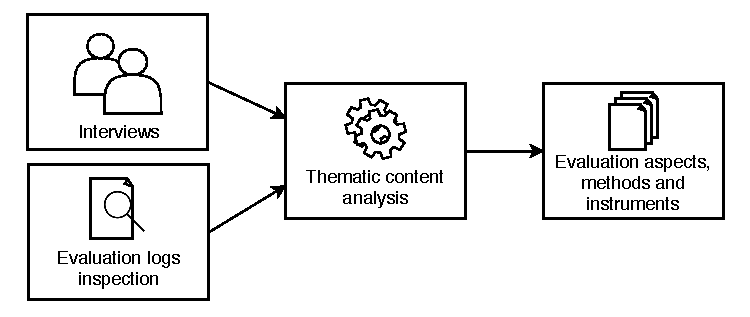
\includegraphics[width=\linewidth]{gfx/aspects/aspectsIdentification}} \quad
\caption{Aspects, methods and instruments identification process}\label{fig:aspectsIdentification}
\end{figure}

\subsection{Analysis}
Collected data is analysed using the thematic analysis method \autocite{Burnard2008}. We produce a list of statements related to the aim of the study. Then, we assign a code to each statement. After that, codes are iteratively grouped to identify potential themes, which are reviewed until defining the four final. 

The initial codes and final themes are presented to the student and three other physiotherapists to validate that the results represented their view. They clarified or added information regarding two statements, though the codes and themes remained the same. The thematic analysis is available online\footnote{Aspects, methods and instruments thematic analysis: \url{https://goo.gl/iJEukN}}.

%-----------------------------------

\section{Aspects, methods and instruments for evaluating PREG}\label{sec:findings_aspects} % Findings -----------------------------------
We identified 46 statements regarding aspects, instruments and methods to evaluate \acp{PREG}. After grouping and categorising the statements iteratively, we identified four final categories: evaluation aspect (31 statements), evaluation instrument (18 statements), evaluation method (8 statements) and evaluation occurrence (1 statement). Some statements belong to more one theme. A summary of teh findings is presented in \autoref{fig:aspectsInstrumentsMethodsIdentificationGraph}.

\begin{figure}[htb]
\myfloatalign
{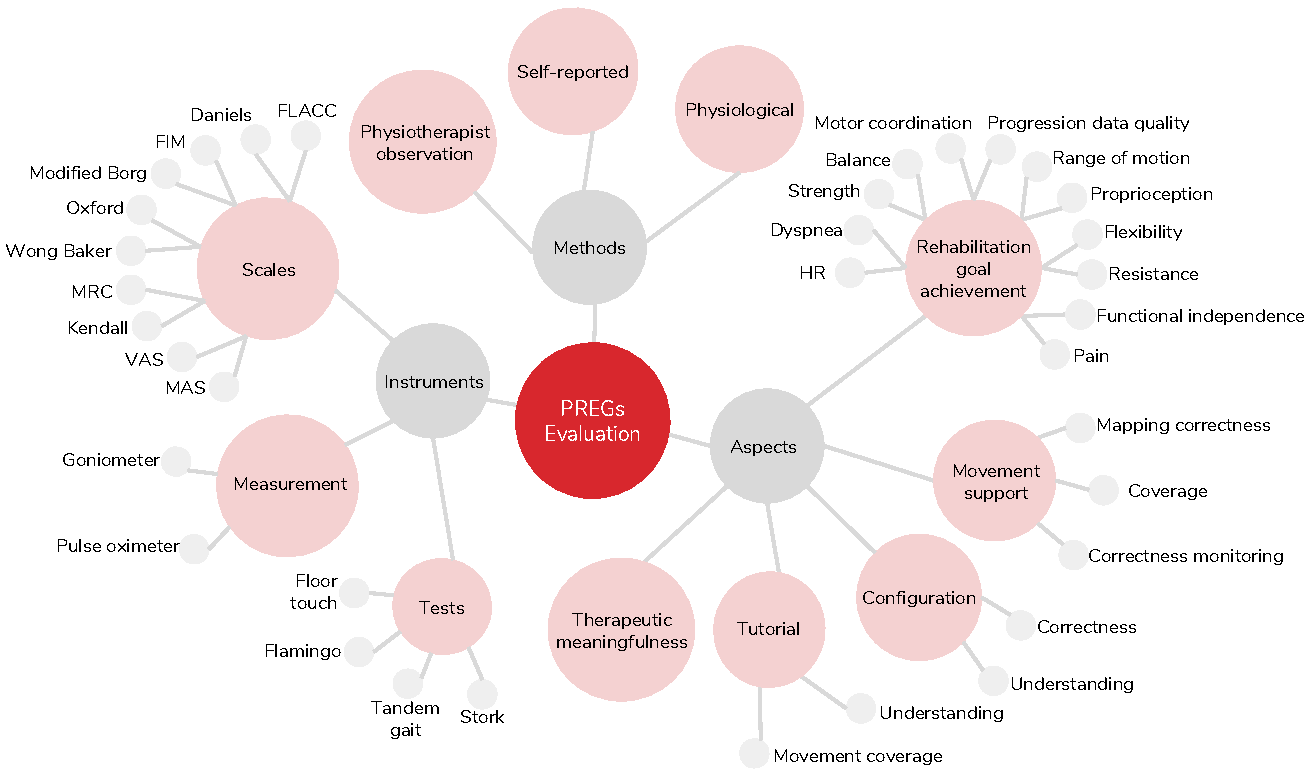
\includegraphics[width=\linewidth]{gfx/aspects/aspectsInstrumentsMethodsIdentificationGraph}} \quad
\caption{Map of qualitative findings, including themes and sub-themes associated to the aspects, methods and instruments identification}\label{fig:aspectsInstrumentsMethodsIdentificationGraph}
\end{figure}

\subsection{Evaluation aspects}
\label{sec:rehab_aspects}
The participants mentioned that the quality of a \ac{PREG} should be measured regarding the impact on patients' progress. They remarked that the highest expectation of patients is to finish their therapies as soon as possible to return to their daily life activities. They highlighted that when a physiotherapist includes something new into the therapy, a patient expects it to be meaningful to their rehabilitation progress. Accordingly, they mentioned different aspects that would allow assessing patients' progress using a \ac{PREG}. These aspects include the range of motion, functional independence, resistance, strength, \ac{HR}, dyspnea, balance, motor coordination, proprioception, flexibility and pain. The selection of aspects to evaluate may depend on the sought after therapeutic goal.

The student validated the correctness of the configuration parameters of each mini \ac{PREG}; i.e., that the configuration parameters produce the expected behaviour. She tested all possible game modes (e.g. movements modes) and verified that each movement was mapped or represented correctly in the mini \ac{PREG}. She suggested including new movements for some mini \acp{PREG}.

Moreover, she assessed that the phrasing of all configuration parameters was understandable for patients and physiotherapists. Furthermore, she tested the relevance of the audiovisual feedback provided by each \ac{PREG} regarding movement correctness.

The student reviewed all mini \acp{PREG}' tutorial; she verified that the phrasing of all instructions was understandable, that all the associated movements were explained and related to a game mechanic. She suggested explaining all movements using graphics and animations.

\subsection{Evaluation methods}
\label{sec:rehab_methods}
The interviews allowed us to identify the following three types of methods for evaluating rehabilitation aspects:

\begin{enumerate}
  \item \emph{Physiotherapist observation}: the evaluation of an aspect depends on the physiotherapist's observation and the criteria of the instrument being employed. For instance, when physiotherapists assess the balance of a patient using the flamingo test \autocite{flamingo}. 
  \item \emph{Self-reported}: patients rate an aspect subjectively, and physiotherapists establish conclusions according to the employed instrument. For instance, patients can rate the pain intensity they are feeling using a \ac{VAS} \autocite{vasScale}.
 \item \emph{Physiological}: physiotherapists collect data directly from patients body; e.g. when they measure the range of motion of a joint.
\end{enumerate}

\subsection{Evaluation instruments}
\label{sec:rehab_instruments}
The participants mentioned some physiotherapy instruments that can be used to evaluate some of the rehabilitation aspects mentioned above. Interviewed physiotherapists expressed that they use the Daniels \autocite{danielsScale}, the \ac{MAS} \autocite{ashwortScale}, the Kendall \autocite{kendallScale}, the Oxford \autocite{oxfordScale} and the \ac{MRC} \autocite{mrcScale} scales to assess muscle strength. They measure pain using the \ac{VAS} \autocite{vasScale}, the \ac{FLACC} \autocite{flaccScale} and the Wong-Baker FACES \autocite{Baker} scales. Also, they use the pulse oximeter to measure \ac{HR} and oxygen saturation. They use the Modified Borg Scale \autocite{modifiedBorgScale_2014} to assess perceived exertion and dyspnea (i.e., shortness of breath). Finally, they expressed that they used the \ac{FIM} \autocite{fim} to assess patients' functional independence and the goniometer \autocite{goniometry} to measure the range of motion. 

Furthermore, they mentioned three tests to assess balance; i.e., the flamingo test \autocite{flamingo}, the tandem gait test \autocite{tandemGaitTest} and the stork test \autocite{storkTest}. The student said that the floor touch test \autocite{floorTouch} can be used to assess flexibility. 

The selection of instruments depends on the therapeutic goal of the evaluated \ac{PREG}. Also, some instruments are of private use, which means that each health institution may have different instruments.

\subsection{Evaluation occurrence}
The physiotherapist expressed that evaluations occur before, during and after therapies take place. That allows diagnosing patients health status and tracking their progress. 

\section{Current practices}\label{sec:current_aspects}

We reviewed 20 published evaluations of \acp{PREG} (or related digital games) to identify evaluation aspects, instruments and methods by frequently employed by evaluators. 16 evaluations assessed \acp{PREG}, \autocite{Celinder2012,Deutsch2011,Rand2008,Brokaw2015,Burke2009,Chang2011,Fitzgerald2008,Hernandez2013,McNeill2012,Ni2014,PirovanoAdvisor2012,Saposnik2010,Seo2016,Shin2014,Sugarman2009,Wuest2014} and 4 assessed digital games for exercise promotion \autocite{Berkovsky2010,Sinclair2010,Zhang2011,Moran2015}.

The most evaluated aspects were enjoyment \autocite{Sinclair2007,Ni2014,Hernandez2013,Berkovsky2010,Shin2014,Moran2015,Chang2011,Rand2008,McNeill2012}, usability \autocite{PirovanoAdvisor2012,Ni2014,Brokaw2015,Rand2008,Fitzgerald2008,McNeill2012}, ease of use \autocite{Wuest2014,PirovanoAdvisor2012,Hernandez2013,Moran2015,Burke2009,Seo2016}, motivation \autocite{Ni2014,Brokaw2015,Shin2014,Chang2011,Seo2016,McNeill2012}, feasibility \autocite{PirovanoAdvisor2012,Sugarman2009,Shin2014,Rand2008,Saposnik2010} and acceptance \autocite{Wuest2014,PirovanoAdvisor2012}. Additional to feasibility and acceptance, we identified 22 new evaluation aspects including perceived exertion \autocite{Berkovsky2010,Chang2011,Rand2008,McNeill2012}, intention to use \autocite{Wuest2014,Moran2015}, adherence \autocite{Wuest2014,PirovanoAdvisor2012}, anxiety \autocite{Moran2015}, clinical score tracking \autocite{Seo2016} and invasiveness \autocite{McNeill2012}.

Regarding evaluation methods, evaluators prefer using ad-hoc questionnaires \autocite{Sinclair2007,Zhang2011,Wuest2014,PirovanoAdvisor2012,Ni2014,Brokaw2015,Hernandez2013,Berkovsky2010,Shin2014,Rand2008,Burke2009,Seo2016}. Also, the \ac{FMA} \autocite{FMAscale} was employed in \autocite{Brokaw2015,Shin2014,Seo2016}, the \ac{ARAT} was employed in \autocite{Shin2014,McNeill2012} and the Modified Borg scale in \autocite{Rand2008,McNeill2012}. Moreover, we identified 19 new instruments including the Berg Balance Scale \autocite{bergScale}, the \ac{MBI} \autocite{mbiScale}, the Motricity Index \autocite{motricityIndex}, the Presence questionnaire \autocite{Witmer2005} and the \ac{TAM} \autocite{Davis1989}.

Finally, the most employed methods include interview \autocite{PirovanoAdvisor2012,Ni2014,Brokaw2015,Celinder2012,Hernandez2013,Shin2014,McNeill2012}, physiotherapy/clinical tests \autocite{Wuest2014,PirovanoAdvisor2012,Brokaw2015,Sugarman2009,Shin2014,Saposnik2010}, physiotherapy/clinical scales \autocite{Brokaw2015,Berkovsky2010,Rand2008,Fitzgerald2008,Saposnik2010} and field observation \autocite{Brokaw2015,Celinder2012,Shin2014,Chang2011}.

The details of each evaluation and the complete list of identified aspects, instruments and methods are available online\footnote{Frequently evaluated aspects, instruments and methods \url{https://goo.gl/EbVGEb}}.

% -----------------------------------------------

\section{Discussion}\label{sec:discussion_aspects} % Discussion %-----------------------------------------------
The aim of this study is to identify aspects that physiotherapists consider important to evaluate \acp{PREG}. Based on the findings, we confirmed that there are rehabilitation aspects that evaluators should consider to assess the impact of \acp{PREG} on patients' treatments. We identified a set of aspects related to rehabilitation goal achievement, movement support, configuration capability, tutorial quality (i.e., user guidance) and therapeutic meaningfulness. Those aspects are relevant to assess if a \ac{PREG} meets physiotherapists and patients needs, and can be used effectively as an assisting methodology in physical therapy. Additionally, we identified a set of methods and instruments to assess those aspects. Additionally, we complemented our findings with the results of reviewing 20 published evaluations of \acp{PREG} and digital games for exertion promotion.

% Progression
The participants remarked that \acp{PREG} should add value to the patients' rehabilitation progress. Therefore, \acp{PREG} should enable patients and physiotherapists to track progression regarding the expected rehabilitation goal. That may imply tracking performance measurements per session; e.g., maximum achieved movement angles or the success rate of correct executed movements. Also, the quality of the tracked data should be assessed. Those results confirm that clinical score tracking is a relevant feature of a rehabilitation game as claimed in \autocite{Seo2016,PirovanoAdvisor2012}.

% Configuration
Additionally, our findings suggest that the configuration capability of \acp{PREG} is important for physiotherapists. According to the student logs, configuration parameters should cover all movements associated with the \ac{PREG}, and the correctness may be assessed by a physiotherapy expert. The configuration capability is relevant since it allows personalising a gameplay session according to a patients' needs, which is important to ensure patients' safety as concluded in \autoref{ch:characterising} and in \autocite{Cameirao2010,Ni2014,Nijholt2008,Wiemeyer2015,Seo2016}.

Additionally, the configuration parameters of a \ac{PREG} should be understandable and easy to use for physiotherapists. In that context, evaluators should assess aspects such as satisfaction \autocite{Sanchez2009,Yanez-Gomez2017,Zhao2016}, ease of use \autocite{Cameirao2010,Moosajee,VandenAbeele2016}, learnability \autocite{Desurvire2009,GonzalezSanchez2009} and acceptance \autocite{Yanez-Gomez2017} involving physiotherapists.

% Associated movements
The physiotherapists and the student's logs suggested that some aspects regarding the \textit{associated movements} of a \ac{PREG} are important. First, movement mapping correctness should be assured since \acp{PREG} use patients' body movements to enable interaction. Second, all movements should be covered by the game mechanics, and patients should consider those movements as meaningful; i.e., the movements should be aligned with the game and therapeutic goals. In that context, evaluators might consider aspects such as accomplishment \autocite{Cameirao2010,Zhao2016} and clarity of goals \autocite{Desurvire2009,VandenAbeele2016}. Third, movement correctness monitoring should be enabled or facilitated by the \ac{PREG}. If the \ac{PREG} is unsupervised, feedback about movement correctness should be automatic, immediate, realistic and specific \autocite{Pasch2009,PirovanoAdvisor2012,Wiemeyer2015}. Otherwise, physiotherapists may need to be able to interrupt gameplay to correct patients. Also, input devices such as motion sensors should enable a meaningful mapping of rehabilitation movements \autocite{Isbister2015}. Finally, the point of view of a \ac{PREG} should allow patients to identify the outcomes of their actions easily.

%Tutorial, ease of use
The tutorial inspection of the student suggests that \acp{PREG} should help patients understand the game goals and rehabilitation movements effectively. That is, patients' attention should be focused on achieving game goals and not on learning how to control the \ac{PREG} \autocite{Isbister2015,Sinclair2007}. Thus, evaluators should assess aspects such as ease of use, learnability \autocite{Desurvire2009,GonzalezSanchez2009}, cognitive load, attention \autocite{Fernandez2008}, clarity of goals \autocite{Desurvire2009,VandenAbeele2016} and absorption \autocite{Lapas2015}. Additionally, the tutorial should cover all associated movements and explains their relation to game mechanics. The quality of tutorials levels should be assessed since patients may have different literacy levels as described in \autoref{sec:reh_patients_constraints}.

%finish as soon as possible, motivation to return to daily life
As expected, the results indicated that \acp{PREG} should be meaningful to patients physical progress. Thus, evaluators should evaluate the capability of \acp{PREG} to contribute to the achievement of the rehabilitation goal. It can be assessed by using the identified rehabilitation aspects, instruments and methods, which are selected depending on the rehabilitation goal. However, evaluators should consider monitoring a group of patients throughout their whole rehabilitation treatments to asses the impact of a \ac{PREG} on patients recovery process properly.

\subsection{Limitations}
The conducted study has some limitations. First, the findings cannot be generalised since the study was qualitative and the source of information was two people. Also, the collected data is based on the experience of the interviewees, one as a physiotherapist and the other as a \ac{PREG} developer (tester). Consequently, there should be more aspects, methods and instruments that may affect the evaluation of \acp{PREG}. Nonetheless, we tried to overcome this limitation by complementing our findings with the information of 20 published evaluations. Finally, most of the results apply to supervised \acp{PREG} since both interviewees based their answers on the idea of including \acp{PREG} in physical therapies at a hospital.

% -----------------------------------------------

\section{Conclusion}\label{sec:conclusion_aspects} % Conclusion -----------------------------------------------
This chapter presented a qualitative study to identify relevant aspects to evaluate \acp{PREG} from the physiotherapy perspective. We confirmed that \ac{GUR} aspects are not sufficient to evaluate \acp{PREG} properly. Evaluators should evaluate if a \ac{PREG} meets physiotherapists and patients expectations and needs. As a result, additional aspects related to the rehabilitation goal assisted by a \ac{PREG} should be assessed; e.g. rehabilitation goal achievement, movement mapping correctness, configuration capability, safety and progress feedback. Also, the ease of use and understanding of the configuration parameters is important to meet physiotherapists expectations. Finally, the ease of use of \acp{PREG} is relevant to avoid patients' distraction from rehabilitation goal. We also identified instruments and methods that may allow evaluating rehabilitation aspects. The findings presented limitations since the conducted study is qualitative and the number of participants is low.